\documentclass[../Head/Main.tex]{subfiles}
\begin{document}

\subsection{Effectiveness of LIDAR line detection}

The purpose of this test is establish the effectiveness of the line detection algorithm for the LIDAR sensor.

\subsubsection*{Description of test}
The initial position of the robot for this test is the origin of the environment \texttt{bigworld}. Here the robot is steered around in the environment using the keypad. The idea of this test is to test if all marbles detected by the algorithm actually corresponds to marbles in the environment.     

\subsubsection*{Test parameters}
\begin{tabular}{l r}
	- World used                & bigworld\\	
	- Number of spawn marbles   & 20\\
	- Number of tests           & 9\\
	- Angle between two found lines & 0.1\\
	- Angle from start/end point to closest line that strikes the marble & 0.5\\
	- Angle between previous and current linemodel $\theta_{max}$ & 0.0025 \\
	- Angle between two points relative to the robot $\Delta\theta$ & $\left(\theta_0 - \theta_1\right) \cdot 1.25$ 
\end{tabular}

\subsubsection*{Data}
\begin{figure}[H]
  \begin{subfigure}[b]{0.3\textwidth}
  	\centering
    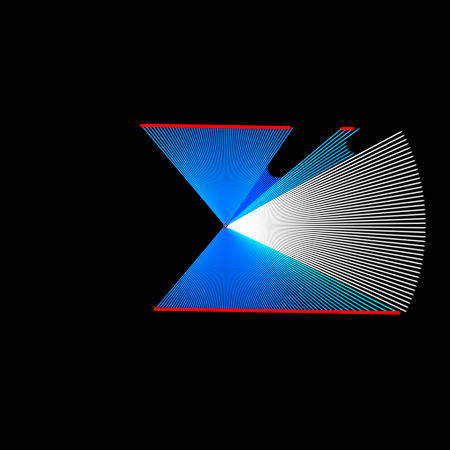
\includegraphics[width=1\textwidth]{Lidar/Test_1_lines}
    \caption{Illustration of data for test 1}
    \label{fig:Linestest1}
  \end{subfigure}
  \hfill
  \begin{subfigure}[b]{0.3\textwidth}
  	\centering
    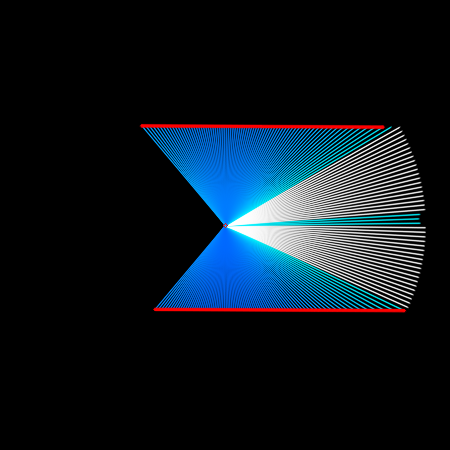
\includegraphics[width=1\textwidth]{Lidar/Test_2_lines}
    \caption{Illustration of data for test 2}
    \label{fig:Linestest2}
  \end{subfigure}
  \hfill
  \begin{subfigure}[b]{0.3\textwidth}
    \centering
    
\includegraphics[width=1\textwidth]{Lidar/Test_3_lines}
    \caption{Illustration of data for test 3}
    \label{fig:Linestest3}
  \end{subfigure}
  \caption{Illustration of data for line detection test 1-3}
  \label{fig:Linestests13}
\end{figure}
\begin{figure}[H]
  \begin{subfigure}[b]{0.3\textwidth}
    \centering
    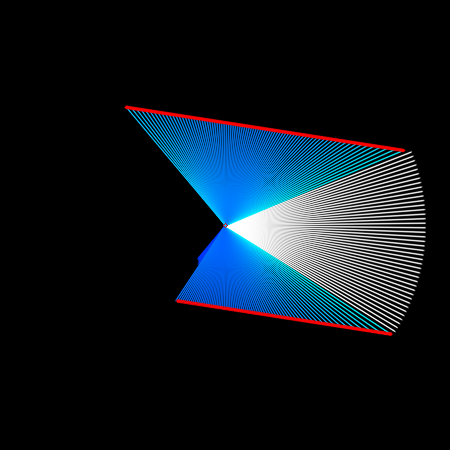
\includegraphics[width=1\textwidth]{Lidar/Test_4_lines}
    \caption{Illustration of data for test 4}
    \label{fig:Linestest4}
  \end{subfigure}
  \hfill
  \begin{subfigure}[b]{0.3\textwidth}
    \centering
    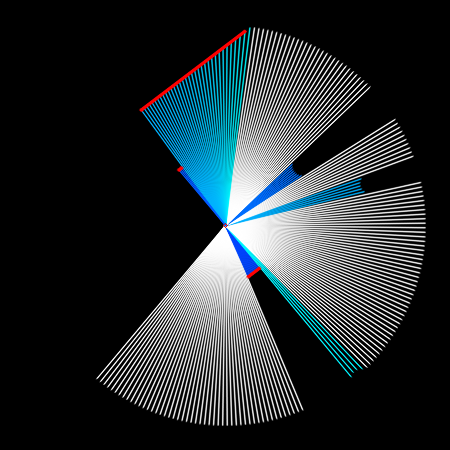
\includegraphics[width=1\textwidth]{Lidar/Test_5_lines}
    \caption{Illustration of data for test 5}
    \label{fig:Linestest5}
  \end{subfigure}
  \hfill
  \begin{subfigure}[b]{0.3\textwidth}
    \centering
    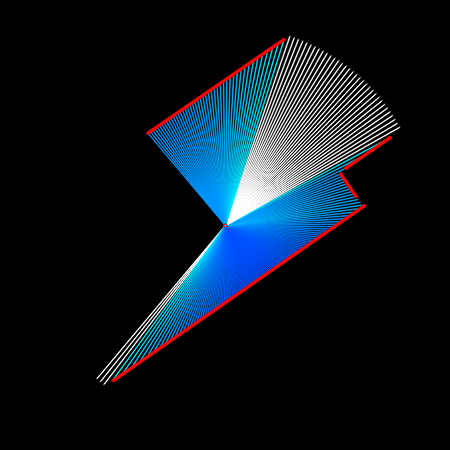
\includegraphics[width=1\textwidth]{Lidar/Test_6_lines}
    \caption{Illustration of data for test 6}
    \label{fig:Linestest6}
  \end{subfigure}
  \hfill
  \begin{subfigure}[b]{0.3\textwidth}
    \centering
    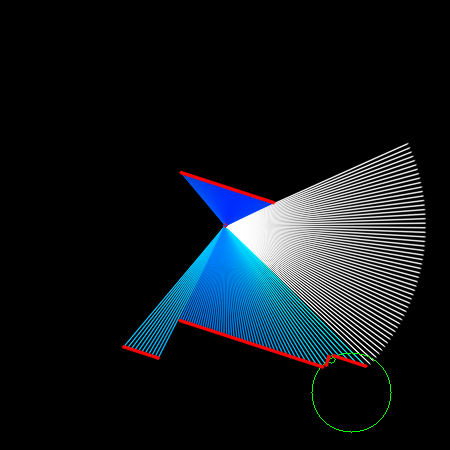
\includegraphics[width=1\textwidth]{Lidar/Test_7_lines}
    \caption{Illustration of data for test 7}
    \label{fig:Linestest7}
  \end{subfigure}
  \hfill
  \begin{subfigure}[b]{0.3\textwidth}
    \centering
    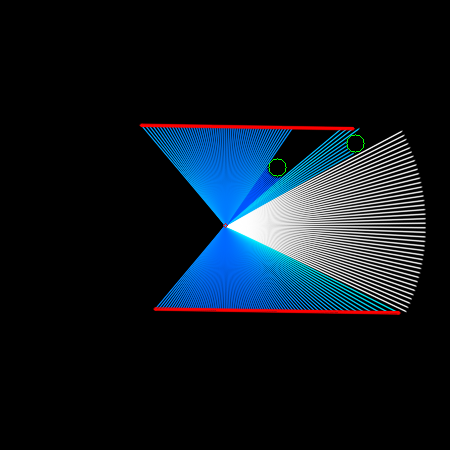
\includegraphics[width=1\textwidth]{Lidar/Test_8_lines}
    \caption{Illustration of data for test 8}
    \label{fig:Linestest8}
  \end{subfigure}
  \hfill
  \begin{subfigure}[b]{0.3\textwidth}
    \centering
    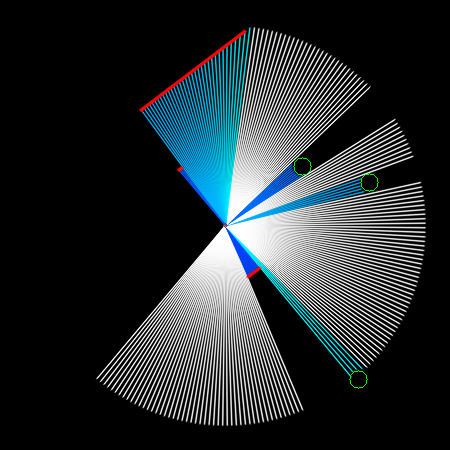
\includegraphics[width=1\textwidth]{Lidar/Test_9_lines}
    \caption{Illustration of data for test 9}
    \label{fig:Linestest9}
  \end{subfigure}
  \caption{Illustration of data for line detection test 4-9}
  \label{fig:Linestests49}
\end{figure}

\subsubsection*{Conclusion}
It can be concluded that the line detection algorithm is reliable, since it all obstacles such as wall in all tests. 
\end{document}